\documentclass[12pt,a4paper]{report}
\usepackage[utf8]{inputenc}
\usepackage[T1]{fontenc}
\usepackage{graphicx}
\usepackage{geometry}
\usepackage{float}
\usepackage{booktabs}
\usepackage{hyperref}
\geometry{margin=1in}

\title{Smart Automatic Egg Incubator}
\author{Project Team}
\date{\today}

\begin{document}
\maketitle

\begin{abstract}
This report documents the design and prototype development of a microcontroller-based egg incubator. The proposed system monitors enclosure temperature and uses a relay-controlled heating arrangement, air-circulation fan, LCD interface, and audible alert. Test measurements and final operating results must be inserted from the actual prototype before this report is submitted.
\end{abstract}

\tableofcontents

\chapter{Introduction}
Egg incubation requires a suitably controlled environment. This project explores a prototype that monitors temperature and controls a heating arrangement using a microcontroller.

\chapter{Problem Statement}
Manual monitoring and adjustment of an incubator can require frequent attention. Temperature variation may occur if the environment is not monitored and controlled consistently. The project investigates a compact, low-cost automated monitoring and control approach.

\chapter{Objectives}
\begin{itemize}
  \item Develop a compact incubator enclosure.
  \item Monitor internal temperature using a digital sensor.
  \item Display readings on an I2C LCD.
  \item Control heating through a relay and programmed limits.
  \item Circulate air using a DC fan.
  \item Evaluate the prototype through documented tests.
\end{itemize}

\chapter{Design and Components}
The documented enclosure is approximately $45\,\mathrm{cm}\times45\,\mathrm{cm}$; the third dimension and internal dimensions should be verified. The reported components include Arduino Nano, DHT22 sensor, I2C LCD, relay module, buzzer, 12 V DC fan, and a PTC heating element. The final heater rating and electrical arrangement must be verified against the assembled prototype.

\section{Internal Arrangement}
The egg tray is supported above the lower compartment. A DC fan is mounted on a side panel. The final location of the heater and electronics should be documented with actual photographs and a wiring diagram.

\begin{figure}[H]
\centering
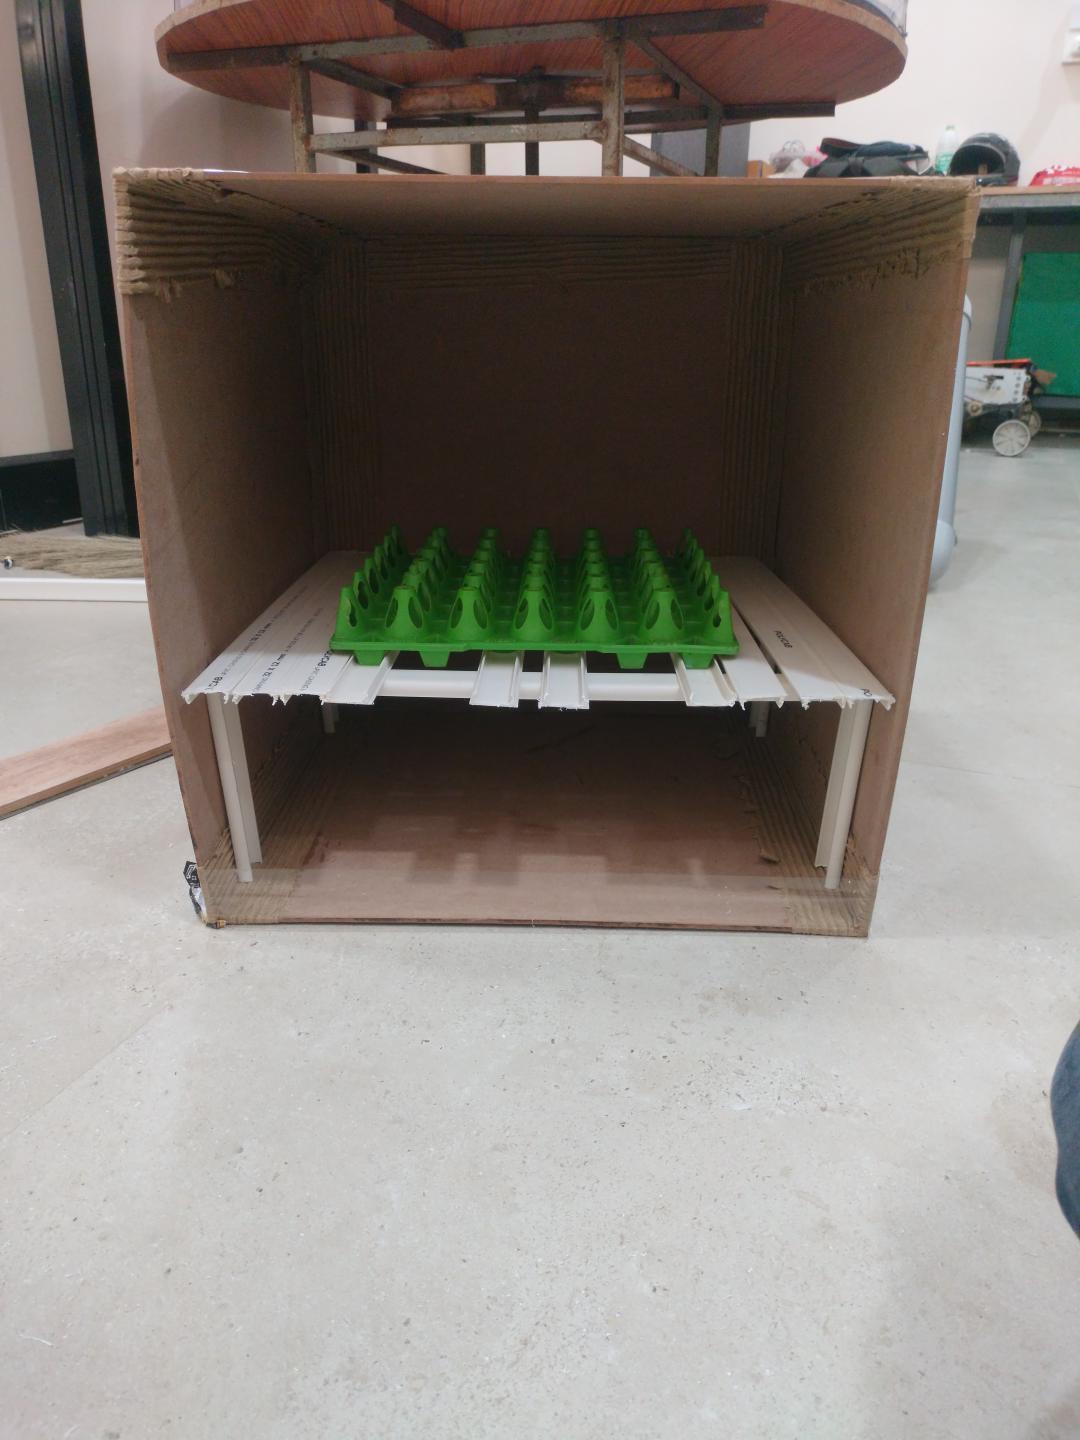
\includegraphics[width=0.75\textwidth]{../assets/images/assembly/egg_tray_internal_structure.jpeg}
\caption{Internal support structure and egg-tray placement.}
\end{figure}

\section{Enclosure Fabrication}
The following photograph records a workshop fabrication and assembly stage.

\begin{figure}[H]
\centering
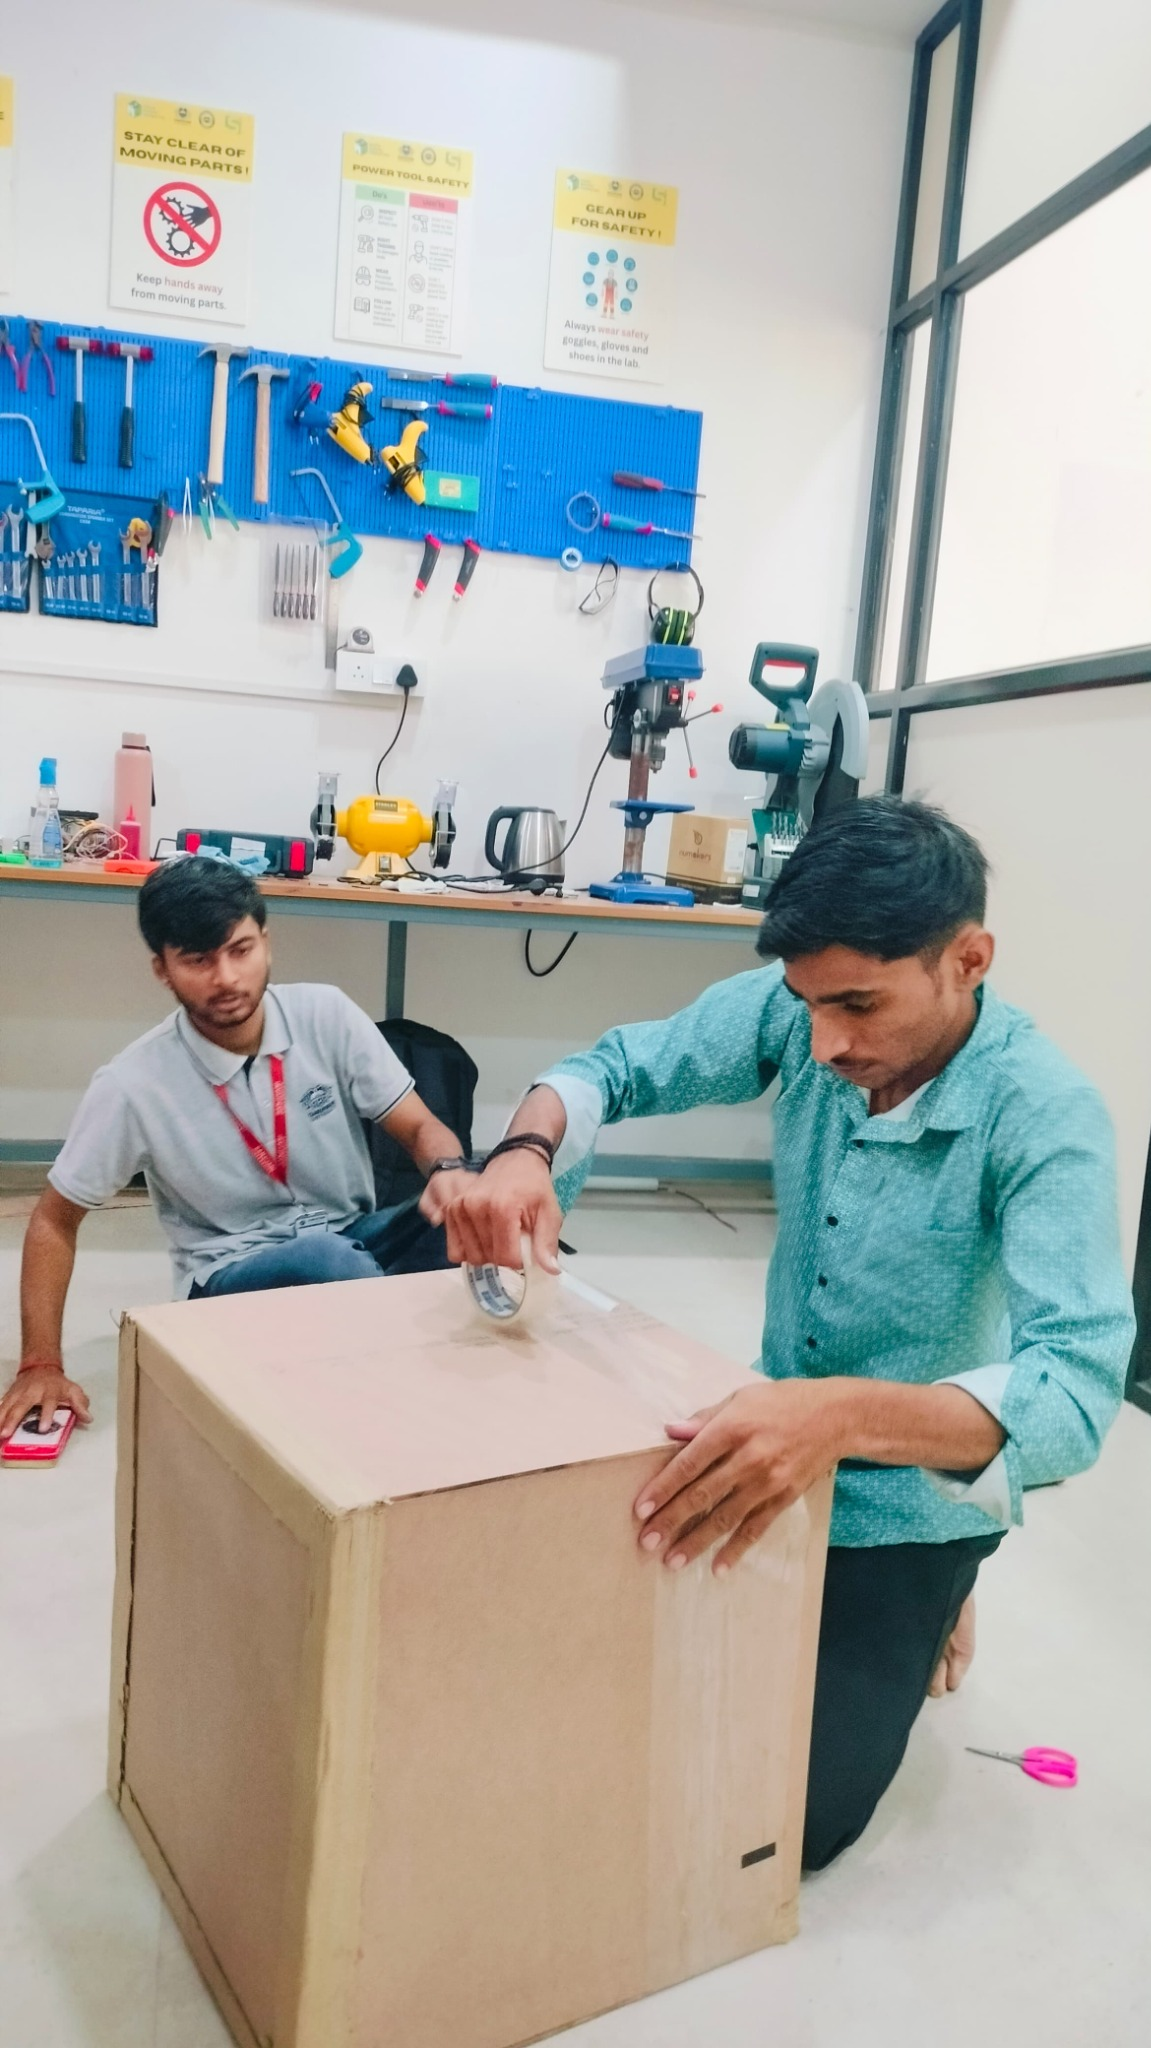
\includegraphics[width=0.75\textwidth]{../assets/images/design_and_fabrication/incubator_box_fabrication.jpeg}
\caption{Fabrication and assembly of the incubator enclosure.}
\end{figure}

\chapter{Working Principle}
The sensor measures the enclosure temperature and sends readings to the Arduino. The controller displays the reading and compares it with programmed limits. Based on the verified control logic, the relay switches the heating circuit. A fan circulates air, and a buzzer may provide an alert under programmed conditions. Exact thresholds and pin assignments must match the final source code.

\chapter{Fabrication and Assembly}
Describe the actual cutting, joining, mounting, wiring, and assembly steps here. Add only steps that were performed and support them with original evidence.

\chapter{Testing and Results}
\textbf{Important:} Insert actual measurements from the prototype. Do not invent test results.

\begin{table}[H]
\centering
\begin{tabular}{p{0.34\textwidth}p{0.48\textwidth}}
\toprule
Test & Observation / measured result \\
\midrule
Temperature sensor accuracy & To be measured \\
LCD operation & To be verified \\
Relay switching & To be verified \\
Heater temperature rise & To be measured \\
Air temperature uniformity & To be measured \\
Temperature stability & To be measured \\
Buzzer operation & To be verified \\
\bottomrule
\end{tabular}
\caption{Prototype test record template.}
\end{table}

\chapter{Conclusion}
The project establishes a prototype platform for temperature monitoring and relay-based heating control in an incubator enclosure. Final conclusions about temperature stability, reliability, and incubation performance can only be made after the relevant tests have been completed and documented.

\chapter{Future Work}
Possible next steps include completing and verifying the heater installation, measuring temperature at multiple locations, improving insulation and airflow if required, adding data logging, and conducting a supervised incubation trial with recorded outcomes.

\chapter{Safety}
The heater and electrical system must be tested with appropriately rated wiring, switching devices, fuse protection, secure mounting, and suitable separation from combustible materials. The prototype should be supervised during powered testing.

\end{document}
